\chapter{JavaScript-ohjelman muuttaminen staattisesti tyyppitarkastetuksi}

\section{Tyyppiannotaatiot}

Tyyppijärjestelmä voi päätellä muuttujan sallitun tyypin automaattisesti
päättelemällä tai kieleen sisältyvien eksplisiittisten tyyppimäärittelyjen
perusteella. Kaikki kolme tässä tutkielmassa esiteltyä JavaScriptin staattiseen
tyyppitarkastukseen tarkoitettua työkalua päättelevät muuttujien tyyppejä automaattisesti,
mutta vaativat paikoitellen myös eksplisiittisiä määrityksiä.
Closure-kääntäjä lukee
tyyppimääritykset JSDoc-tyylisistä dokumentaatiokommenteista \cite{annotatingJSforClosure}.

\begin{minipage}{\linewidth}
\begin{lstlisting}[caption={Esimerkki Closure-annotaatiosta funktiolle},label={lst:ostoskorin_hinta_closure}]
/**
* @param {!Array<Ostos>} ostokset
* @return {number} Ostosten yhteenlaskettu hinta
*/
function ostoskorinHinta(ostokset) {
  let summa = 0;
  for (const ostos of ostokset) summa += ostos.hinta;
  return summa;
}
\end{lstlisting}
\end{minipage}
Listauksessa \ref{lst:ostoskorin_hinta_closure} \inlinecode{ostoskorinHinta}-funktion
tyyppimäärittely on toteutettu sen yläpuolella olevilla kommenteilla, jotka määrittävät
tyypin \inlinecode{ostokset} parametrille sekä funktion palautusarvolle.
TypeScript ja Flow puolestaan jatkavat ECMA-262 -spesifikaatiota erityisellä syntaksilla
tyyppien eksplisiittistä määrittämistä varten. 

\begin{minipage}{\linewidth}
\begin{lstlisting}[caption={Esimerkki Flow tai TypeScript annotaatiosta funktiolle},label={lst:ostoskorin_hinta_flow}]
function ostoskorinHinta(ostokset: Ostos[]): number {
\end{lstlisting}
\end{minipage}

Flow ja TypeScript -esimerkeissä \ref{lst:ostoskorin_hinta_flow}
tyyppiannotaatiot ovat osana koodia, mikä
tekee ohjelmasta yhteensopimattoman tavallisen JavaScriptin kanssa. Ohjelma
on käännettävä JavaScriptiksi ennen suorittamista. Annotaatioiden
syntaksi ja merkitys ei myöskään ole välttämättä suoraan selvä
JavaScript-ohjelmoijalle, joka pahimmassa tapauksessa voi kokea lisätyt
tyyppimäärittelyt vaikeasti luettavina. 

Closuren annotaatiot on sijoitettu kommentteihin, joten niillä ei ole
ajonaikaista vaikutusta ja ohjelma on täten sellaisenaan hyväksyttävää
JavaScriptiä. Toisaalta tyyppiannotaatioiden määrittely kommenteissa voi
olla runsassanaista ja hankalaa, mikä kasvattaa niiden kirjoittamiseen vaadittua
työmäärää \cite{TypeScriptSpec, TypeScriptatBuild}.

\begin{minipage}{\linewidth}
Aiemmassa esimerkissä esitelty tyyppi \inlinecode{Ostos} pitäisi
määritellä Closurea varten muiden annotaatioiden tapaan dokumentaatiokommentteja käyttäen:
\begin{lstlisting}[label={lst:closure_typedef}]
/**
* @typedef {{
*   nimi: string,
*   hinta: number
* }}
*/
let Ostos;
\end{lstlisting}
\end{minipage}

TypeScript ja Flow tarjoavat käännösaikaisen tyypin (type alias)
määrittelyyn tiiviimmän ja helppolukuisemman syntaksin \cite{TypeScriptSpec}:

\begin{minipage}{\linewidth}
\begin{lstlisting}[label={lst:ts_flow_type_alias}]
type Ostos = {
  nimi: string;
  hinta: number;
};
\end{lstlisting}
\end{minipage}
Tällainen tyypin määritteleminen vaikuttaa ainoastaan käännösvaiheen
tyyppitarkastukseen, eikä määrittely tuota tietorakenteita tai muuta
sisältöä suoritettavaan JavaScript-ohjelmaan.

\section{Ohjelman kääntäminen ennen suorittamista}

JavaScript koodi tulkataan tai käännetään tyypillisesti suorittamisen
yhteydessä, selaimesta tai muusta suoritusympäristöstä löytyvän ”moottorin”
toimesta. EcmaScript-standardin mukaista koodia suorittamaan suunnitellut
moottorit, kuten V8 tai SpiderMonkey, eivät kuitenkaan osaa käsitellä
TypeScript- tai Flow-annotaatioilla merkattua koodia. Näinollen TypeScript-
tai Flow-annotoitu koodi on välttämätöntä kääntää muotoon jossa
annotaatiot on poistettu ja jäljellä on enää standardinmukainen JavaScript.
Koska JavaScriptin käyttäminen ei normaalisti vaadi erillistä
käännösvaihetta, useissa projekteissa ei ole sellaista käytetty. Koodin
minimointi ja muu optimointi on ollut parhaiden käytäntöjen mukaista jo
tovin, mutta tällaiset koodinkäsittelyt tehdään yleensä vasta ennen ohjelman
julkaisua. Kehittäjät ovat tavanomaisesti voineet suorittaa kirjoittamansa
JavaScriptin sellaisenaan kehitysympäristössä. Käännösvaiheen aikavaatimus
pyritään luonnollisesti pitämään mahdollisimman pienenä, mutta se on silti
projektin monimutkaisuuteen ja kehitysnopeuteen vaikuttava tekijä, tulee
tulee huomioida työkalun käyttöönotossa.

\begin{figure}
\centering
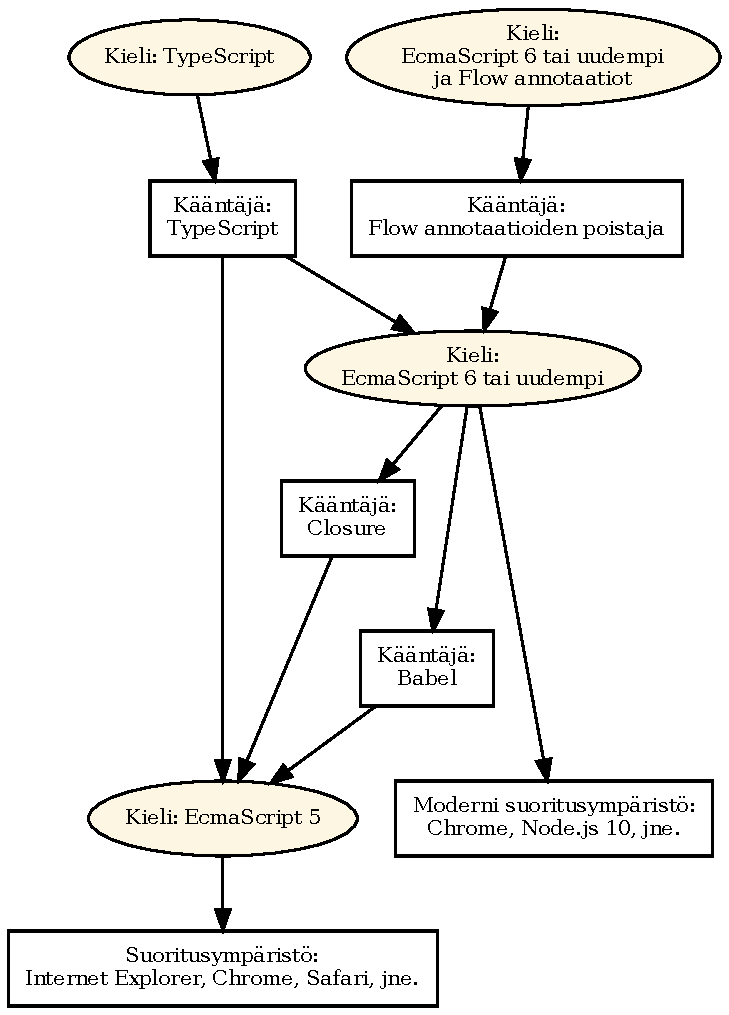
\includegraphics[width=0.6\textwidth]{images/compilation.pdf}
\caption{Vaihtoehtoisia käännösprosesseja}
\label{fig:compilation}
\end{figure}

Kuva \ref{fig:compilation} esittää erilaisia käännösprosesseja eri
JavaScript-ohjelman kehityskielille. Jos koodi kirjoitetaan kaikkiin
suoritusympäristöihin soveltuvalla kielen versiolla, kuten EcmaScriptin
versiolla 5 (2011), käännösvaihe voidaan jättää kokonaan väliin. Kielen
uudemmat versiot ovat kuitenkin tuoneet monia lisäominaisuuksia, joiden
käyttäminen vanhempia selaimia tukevissa ohjelmissa vaatii joka tapauksessa
käännösvaiheen staattisesta tyypittämisestä riippumatta. Uusia JavaScript-
ominaisuuksia hyödyntäville projekteille koodin kääntäminen ei siis tule
täysin uutena vaiheena.

\section{Työkalun vaiheittainen käyttöönotto}

JavaScript-kirjastojen hallintaan tarkoitettu rekisteri npm on yksi
suurimmista ohjelmistoekosysteemeistä \cite{DynamicsOfJSPackages}.
Tutkinnon kirjoittamisen hetkellä rekisterin kotisivu, npmjs.com ilmoitti
ladattavissa olevien pakettien määräksi yli 595 000. Avoimessa jakelussa
olevien kirjastojen lisäksi JavaScriptiä käyttävillä kehittäjillä voi olla
suuri määrä valmista JavaScript-koodia, jota voi hyödyntää uusissa
projekteissa. Jotta TypeScript, Flow ja Closure olisivat hyödyllisiä
työkaluja JavaScript-ohjelmien kehitykseen, on niiden oltava yhteensopivia
sellaisen JavaScript-koodin kanssa jonka kehitykseen ei kyseistä työkalua
ole käytetty.

TypeScript ja Flow tukevat erityisiä määrittelytiedostoja, joiden sisältämällä
tyyppiannotoidulla koodilla määritetään kirjaston tai muun JavaScript-koodin
ulkoisen rajapinnan tyyppimäärittelyt. Näiden tiedostojen kirjoittamiseen
käytetty syntaksi on muuten sama kuin muissakin tiedostoissa, muuta niiden funktio- ja
metodimäärittelyistä on jätetty implementaatiot kokonaan pois. Tiedoston ei
ole tarkoitus olla osana varsinaista suoritettavaa koodia, vaan se palvelee
ainoastaan kuvauksena sellaisen koodin tyyppimäärittelystä, jonka käsittelyä
TypeScript ja Flow eivät muuten voisi valvoa. TypeScriptillä voitaisiin
esimerkiksi kirjoittaa seuraava tiedosto \inlinecode{ostoskori.d.ts}, jonka
tehtävä on annotoida toista tiedostoa \inlinecode{ostoskori.js}.

\begin{minipage}{\linewidth}
\begin{lstlisting}[caption={Esimerkki TypeScript määrittelytiedostosta ostoskori.d.ts}]
/** Laittaa tuotteen ostoskoriin. */
export function lisaaTuote(ostos: Ostos): void;
\end{lstlisting}
\end{minipage}
Tämän jälkeen TypeScript tiedostosta käsin voidaan kutsua tätä
JavaScript-funktiota siten, että TypeScript valvoo
tyyppien oikeellisuutta.

\begin{minipage}{\linewidth}
\begin{lstlisting}[caption={JavaScript-koodin kutsuminen TypeScript tiedostosta tuotesivu.ts}]
import * as ostoskori from "./ostoskori";

ostoskori.lisaaTuote({ nimi: "juusto", hinta: 5 });
\end{lstlisting}
\end{minipage}

Joissain tapauksissa kirjastoille tai kehittäjän omalle aiemmin kirjoitetulle
JavaScript koodille ei kuitenkaan ole valmiita TypeScript-tyyppimäärittelyjä
eikä niitä syystä tai toisesta voida luoda ennen muun kehityksen jatkamista.
Kaikkien kolmen työkalun tärkeimpiin ominaisuuksiin kuuluu tuki vaiheittaiselle
käyttöönotolle, eli käytännössä yhteenspivuus täysin tyyppitarkastamattoman
koodin kanssa. Sekä Flow että TypeScript tarjoavat erityisen
yleisviittaustyypin Any, jota voi käyttää kuvaamaan mitä tahansa JavaScript
arvoa \cite{TypeScriptSpec}. Any-tyyppiseen muuttujaan voidaan asettaa mikä
tahansa arvo ja Any tyyppinen arvo voidaan asettaa mihin tahansa muuttujaan
tai funktioparametriin. Any tyypin avulla muuten staattisesti tyypitetyssä
ohjelmassa voidaan ohittaa käännösaikainen tyyppien tarkistaminen sellaisten
koodin osien kohdalla joiden ajonaikaista arvoa olisi muuten vaikea tai
mahdotonta määritellä käännösaikana. Näin ollen, mikäli tarve vaatii täysin
annotoimattoman JavaScript moduulin käyttämistä, kaikkien kyseisestä moduulista
tuotujen arvojen voidaan määrittää olevan tyyppiä Any, jolloin tarkastaja ei
kiinnitä huomiota siihen miten JavaScriptillä määritettyjä funktioita tai
muita arvoja käsitellään.